\documentclass[pmlr]{jmlr}% PMLR format (Deep Learning Indaba / JMLR-PMLR guidelines)
% jmlr auto-loads: amsmath, amssymb, natbib, graphicx, url, algorithm2e.

\usepackage{booktabs}
\usepackage{float}
\usepackage{tikz}
\usetikzlibrary{positioning,shapes.geometric,arrows.meta,calc}
\graphicspath{{figures/}}
\newcommand{\acc}{\mathrm{Acc}}

\jmlrvolume{}
\jmlryear{2026}
\jmlrworkshop{Trustworthy AI Workshop, Deep Learning Indaba 2026}

% Remove the first-page copyright footer, and the running header on pages 2+.
\makeatletter
\renewcommand*{\@titlefoot}{}
\makeatother

\title[Confidently Wrong: Calibration Risks in LLMs for African Languages]{Confidently Wrong: Measuring and Mitigating Calibration Risks in LLMs for African Languages}

% Anonymized for double-blind review.
\author{\Name{Anonymous Author(s)}}

\begin{document}

\maketitle
\thispagestyle{jmlrtps}% keep the PMLR line on page 1
\pagestyle{plain}% no running header on pages 2+ (page numbers only)
\vspace{-2.2em}% tighten the gap between authors and abstract

\begin{abstract}
Large language models (LLMs) are increasingly used in African languages, yet little is known about
whether their confidence remains reliable. This creates a safety risk: models may become less
accurate while remaining highly confident, increasing the likelihood of trusted misinformation. We
evaluate four open-weight LLMs (\textbf{Qwen3-4B-Instruct}, \textbf{Gemma-4-12B},
\textbf{Aya-Expanse-8B}, and \textbf{AfroLlama-V1}) on African-language truthfulness and knowledge
benchmarks (\textbf{Uhura-TruthfulQA} and \textbf{AfriMMLU}), measuring calibration using
log-probability-based confidence estimates. We find that models become increasingly confident in
incorrect answers as they move from English to African languages, creating a systematic
overconfidence problem and a marked increase in expected calibration error. Among three mitigation
strategies, temperature scaling proves most effective, reducing calibration error to near-English
levels without retraining. Our findings suggest that African-language deployment risks stem not only
from lower accuracy but also from models remaining confident when wrong, and that simple post-hoc
recalibration offers a practical deployment-time safety intervention.
\end{abstract}

\section{Introduction}
LLMs are entering high-stakes, information-seeking use in African languages such as health, legal,
educational, and civic information, often where users cannot easily verify an answer. The safety
failure we study is a mismatch between confidence and correctness. When models remain highly
confident despite being wrong, they can mislead users into treating incorrect information as
reliable, which is particularly dangerous in high-stakes settings such as health, education, and
civic information. A calibrated model, whose confidence tracks its accuracy, can instead
\emph{abstain}, declining or deferring when uncertain \citep{tomani2024}. If calibration holds in
English but breaks in African languages, the populations least served by current models are most
exposed to confident misinformation. We investigate whether models become increasingly overconfident
in African languages, quantify the extent of this misalignment between confidence and correctness,
and evaluate practical strategies for mitigating it.

\medskip
\noindent\textbf{Our main contributions are:}
\begin{enumerate}\itemsep1pt
  \item An open-weight, reproducible calibration audit of four LLMs on African-language truthfulness
  and knowledge benchmarks, using answer-text log-probabilities to obtain robust confidence estimates
  for instruction-tuned models.

  \item Evidence that calibration degrades substantially from English to African languages, revealing
  systematic overconfidence and a growing mismatch between confidence and correctness across models
  and tasks.

  \item An evaluation of practical mitigation strategies, including temperature scaling, abstention,
  and few-shot prompting, together with a deployment framework showing that lightweight post-hoc
  recalibration is an effective safety intervention for African-language LLMs.
\end{enumerate}

\section{Related Work}
Neural networks are often overconfident, and temperature scaling is a standard single-parameter
post-hoc calibration method \citep{guo2017}; for free-form generation, sampling-based methods such as
semantic entropy estimate uncertainty without labelled data \citep{kuhn2023}. \citet{tomani2024}
show that uncertainty-based abstention improves correctness, reduces hallucinations, and increases
safety, motivating uncertainty estimation as a deployment-time safety mechanism. African-language
evaluation has advanced through human-translated benchmarks, including Uhura for truthfulness and
scientific question answering \citep{uhura} and AfriMMLU within IrokoBench for knowledge evaluation
\citep{irokobench}, alongside models such as AfroLlama \citep{afrollama}. However, prior work has
focused primarily on capability and benchmark performance. To our knowledge, calibration in African
languages, compared across models and paired with mitigation strategies, has not been systematically
studied.

\section{Methods}

\subsection{Models}
We evaluate four open-weight models chosen to span size, multilinguality, and origin: a small
instruction-tuned model, a larger one, a multilingual one, and an Africa-specific one (full
specifications in the separately submitted appendix). Open weights give direct log-probability access
and full reproducibility without proprietary APIs.

\subsection{Datasets}
We use Uhura-TruthfulQA \citep{uhura} (English and six African languages; truthfulness; a variable
number of candidate answers per question) and AfriMMLU \citep{irokobench} (18 languages; knowledge;
four options per question). Because their language sets and tasks differ, we analyse them separately
and never average across them. ``African'' denotes all languages other than English and French.

\subsection{Scoring}
For both datasets we score each option by the length-normalised log-probability of its answer text
(a cloze reading; detailed in the appendix) and take the softmax over options as the model's
confidence. We deliberately avoid letter-logit scoring (reading the next-token probability of
``A''/``B''/``C''/``D''): it silently collapses instruction-tuned models, with Gemma-4 returning
``A'' for 75\% of items and scoring below chance, whereas answer-text scoring collapsed for no model.

\subsection{Metrics}
We report expected calibration error (ECE, 15 bins), overconfidence (mean confidence minus accuracy),
Brier score, error-detection AUROC, and AUARC, the area under the accuracy-rejection curve
(definitions in the appendix).

\subsection{Interventions}
We evaluate three: per-language temperature scaling, selective abstention by per-language confidence
threshold, and 5-shot in-context prompting with examples held out from evaluation (detailed in the
appendix).

\section{Results}
Table~\ref{tab:overview} summarises every model on both datasets; the central finding is the gap
between English and African-language calibration.

\begin{table}[t]\centering\small
\caption{English versus African-language performance, by model and dataset. ``en'' is English and
``afr'' is the mean over African languages; ECE(TS) is pooled ECE after per-language temperature
scaling; AUARC measures abstention quality (higher is better). Models are accurate and calibrated in
English but lose both in African languages, and recalibration restores calibration.}
\label{tab:overview}
\resizebox{\textwidth}{!}{%
\begin{tabular}{llcccccc}
\toprule
\textbf{Model} & \textbf{Dataset} & \textbf{Acc(en)} & \textbf{Acc(afr)} & \textbf{ECE(en)} & \textbf{ECE(afr)} & \textbf{ECE(TS)} & \textbf{AUARC}\\
\midrule
Qwen3-4B-Instruct & Uhura-TruthfulQA & 0.38 & 0.32 & 0.07 & 0.17 & \textbf{0.03} & 0.36\\
Gemma-4-12B       & Uhura-TruthfulQA & 0.33 & 0.34 & 0.21 & 0.26 & \textbf{0.03} & 0.39\\
Aya-Expanse-8B    & Uhura-TruthfulQA & 0.36 & 0.31 & 0.08 & 0.20 & \textbf{0.04} & 0.35\\
AfroLlama-V1      & Uhura-TruthfulQA & 0.29 & 0.33 & 0.18 & 0.13 & \textbf{0.04} & 0.35\\
\midrule
Qwen3-4B-Instruct & AfriMMLU & 0.53 & 0.30 & 0.06 & 0.15 & \textbf{0.02} & 0.35\\
Gemma-4-12B       & AfriMMLU & 0.30 & 0.27 & 0.31 & 0.34 & \textbf{0.07} & 0.29\\
Aya-Expanse-8B    & AfriMMLU & 0.52 & 0.29 & 0.06 & 0.18 & \textbf{0.02} & 0.34\\
AfroLlama-V1      & AfriMMLU & 0.36 & 0.28 & 0.22 & 0.20 & \textbf{0.03} & 0.31\\
\bottomrule
\end{tabular}}
\end{table}

\begin{enumerate}\itemsep2pt
  \item \textbf{Calibration degrades from English to African languages.} Across the models and both
  tasks, ECE and overconfidence are substantially higher in African languages
  (Table~\ref{tab:overview}, Figure~\ref{fig:calib}); models are most overconfident where they are
  least accurate.
  \item \textbf{The accuracy collapse is a knowledge story.} On AfriMMLU the capable models fall from
  about 0.52 (English) to about 0.29 (African, near the 0.25 chance floor). On Uhura accuracy is
  uniformly low (about 0.31) with little English advantage, so Uhura supplies the calibration signal
  and AfriMMLU the accuracy decay.
  \item \textbf{Mitigations are unequal.} Per-language temperature scaling cuts pooled ECE to about
  0.02 to 0.07 for every model (see appendix); abstention helps less, because uncertainty is a weak
  error-ranker (AUROC about 0.55), so AUARC sits only modestly above baseline. Few-shot prompting
  gives small gains for three models and backfires on Gemma (see appendix).
  \item \textbf{Bigger is not safer.} Gemma-4-12B is the worst-calibrated model (ECE up to 0.34) and
  is overconfident across every topic, despite being the largest model we evaluate.
\end{enumerate}

Per-language bootstrap 95\% confidence intervals are reported in the appendix.

\begin{figure}[t]\centering
  \begin{minipage}{0.49\textwidth}\centering
    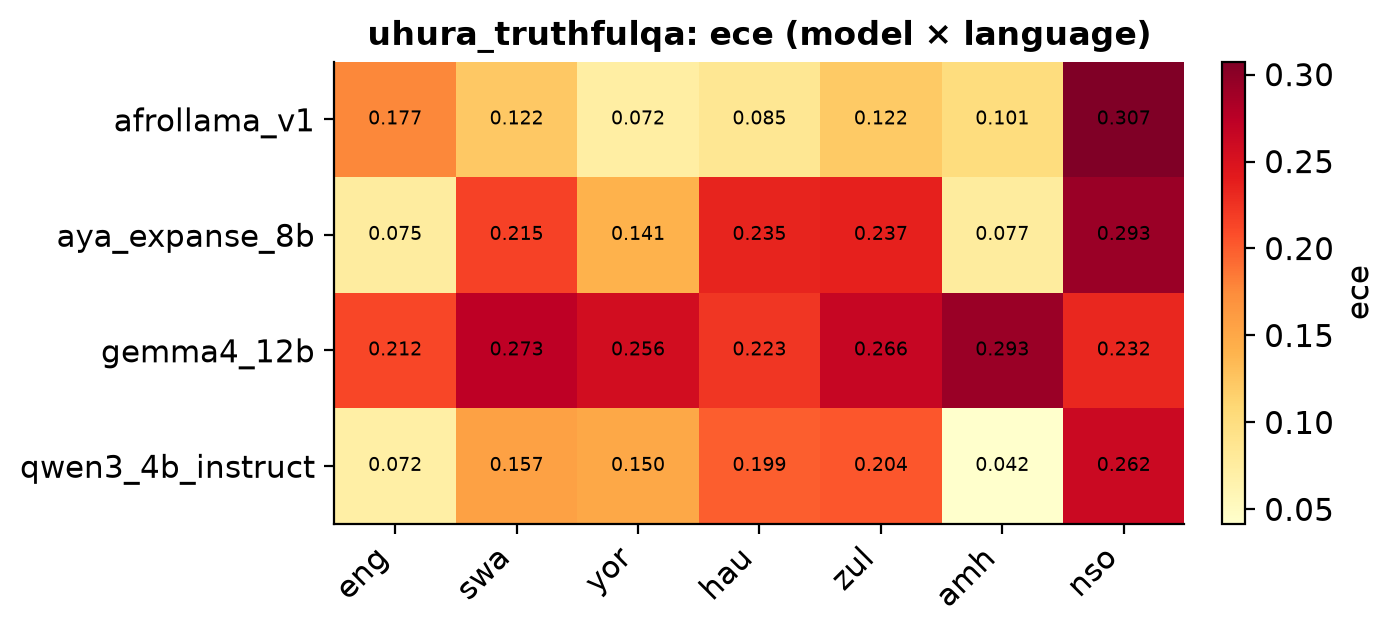
\includegraphics[width=\linewidth]{uhura_ece_heatmap.png}\\[2pt]{\small (a) Uhura-TruthfulQA (7 languages)}
  \end{minipage}\hfill
  \begin{minipage}{0.49\textwidth}\centering
    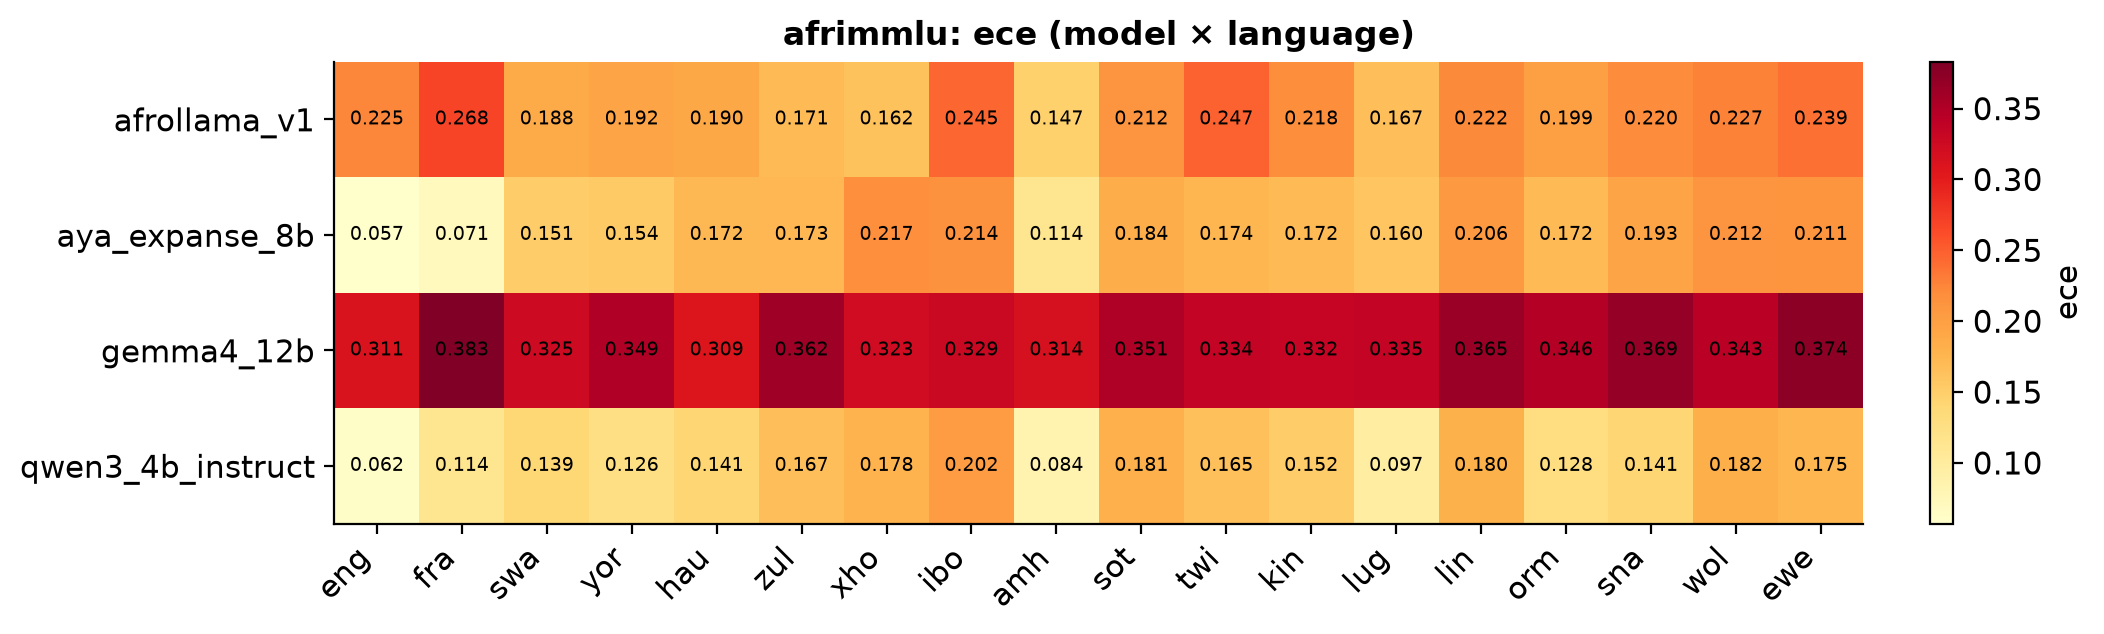
\includegraphics[width=\linewidth]{afrimmlu_ece_heatmap.png}\\[2pt]{\small (b) AfriMMLU (18 languages)}
  \end{minipage}
  \caption{Expected calibration error by model and language. ECE is low in English and French and
  rises across African languages; Gemma is worst throughout.}
  \label{fig:calib}
\end{figure}

\section{Discussion and Limitations}
\textbf{Implications for African AI safety.} In African languages these models are at once less
accurate and more overconfident, the worst combination for trust, since confident wrong answers
reach users precisely where verification is hardest. Encouragingly, much of the failure is an
output-layer problem: cheap, post-hoc, per-language temperature scaling closes most of the
calibration gap with no retraining, so safer deployment is feasible now. Abstention alone is
insufficient because the uncertainty signal is weak, so the durable fix remains better
African-language data and training. We distil this into a deployment framework (detailed in the
appendix): recalibrate, then route on calibrated confidence to answer, ask for more context, or
abstain, logging low-confidence queries for data collection.

\textbf{Limitations.} Accuracies are near chance on these hard, low-resource tasks, so we document
systematic overconfidence rather than catastrophic confident-wrongness, and absolute ECE is moderate
except for Gemma. The weak uncertainty signal (AUROC about 0.55) bounds how much abstention can help.
We cover four open models and two benchmarks; reasoning and frontier closed models were out of scope.

\textbf{Future work.} Reasoning-model and closed-model references; in-context calibration at scale;
the offline data-collection loop in the deployment framework; and human-grounded evaluation of
abstention.

\section{Conclusion}
Open LLMs are confidently wrong in African languages, less accurate and more overconfident than in
English across the models and both tasks. Post-hoc per-language temperature scaling is a cheap,
effective safety lever that closes most of the calibration gap, and our deployment framework pairs it
with thresholded abstention for safer real-world use.

\begin{thebibliography}{9}\small
\bibitem[Guo et al.(2017)]{guo2017} Guo, C., Pleiss, G., Sun, Y., and Weinberger, K. Q. (2017). On
Calibration of Modern Neural Networks. \textit{Proceedings of the 34th International Conference on
Machine Learning (ICML)}, PMLR 70:1321--1330. arXiv:1706.04599.
\bibitem[Kuhn et al.(2023)]{kuhn2023} Kuhn, L., Gal, Y., and Farquhar, S. (2023). Semantic
Uncertainty: Linguistic Invariances for Uncertainty Estimation in Natural Language Generation.
\textit{International Conference on Learning Representations (ICLR)}. arXiv:2302.09664.
\bibitem[Tomani et al.(2024)]{tomani2024} Tomani, C., Chaudhuri, K., Evtimov, I., Cremers, D., and
Ibrahim, M. (2024). Uncertainty-Based Abstention in LLMs Improves Safety and Reduces Hallucinations.
arXiv:2404.10960.
\bibitem[Bayes et al.(2024)]{uhura} Bayes, E., Azime, I. A., Alabi, J. O., Kgomo, J., Eloundou, T.,
Proehl, E., Chen, K., Khadir, I., Etori, N. A., Muhammad, S. H., Mpanza, C., Thete, I. P., Klakow, D.,
and Adelani, D. I. (2024). Uhura: A Benchmark for Evaluating Scientific Question Answering and
Truthfulness in Low-Resource African Languages. arXiv:2412.00948.
\bibitem[Adelani et al.(2024)]{irokobench} Adelani, D. I., et al. (2024). IrokoBench: A New Benchmark
for African Languages in the Age of Large Language Models. arXiv:2406.03368.
\bibitem[Jacaranda Health(2024)]{afrollama} Jacaranda Health (2024). AfroLlama-V1. Hugging Face.
\url{https://huggingface.co/Jacaranda/AfroLlama_V1}.
\end{thebibliography}

\section*{Appendix}
The appendix (model and setup details, metric definitions, prompts, intervention details, the
deployment framework, additional per-language results, reliability curves, and bootstrap confidence
intervals) is provided as a separate PDF file, in compliance with the Trustworthy AI Workshop
(Deep Learning Indaba 2026) submission guidelines.

\end{document}
